% \documentclass[landscape,a0paper,fontscale=0.292]{baposter}
\documentclass[landscape,paperwidth=200cm, paperheight=120cm,fontscale=0.19]{baposter}

\usepackage[vlined]{algorithm2e}
\usepackage{times}
\usepackage{calc}
\usepackage{url}
\usepackage{graphicx}
\usepackage{amsmath}
\usepackage{amssymb}
\usepackage{relsize}
\usepackage{multirow}
\usepackage{booktabs}
\usepackage{subfigure}
\usepackage{bm}

\usepackage{graphicx}
\usepackage{multicol}
\usepackage[T1]{fontenc}
\usepackage{ae}



%%%%%%%%%%%%%%%%%%%%%%%%%%%%%%%%%%%%%%%%%%%%%%%%%%%%%%%%%%%%%%%%%%%%%%%%%%%%%
%% Begin of Document
%%%%%%%%%%%%%%%%%%%%%%%%%%%%%%%%%%%%%%%%%%%%%%%%%%%%%%%%%%%%%%%%%%%%%%%%%%%%%
\begin{document}
%%%%%%%%%%%%%%%%%%%%%%%%%%%%%%%%%%%%%%%%%%%%%%%%%%%%%%%%%%%%%%%%%%%%%%%%%%%%%
%% Here starts the poster
%%---------------------------------------------------------------------------
%% Format it to your taste with the options
%%%%%%%%%%%%%%%%%%%%%%%%%%%%%%%%%%%%%%%%%%%%%%%%%%%%%%%%%%%%%%%%%%%%%%%%%%%%%
\begin{poster}{
 % Show grid to help with alignment
 grid=false,
 % Column spacing
 colspacing=0.7em,
 % Color style
 headerColorOne=cyan!20!white!90!black,
 borderColor=cyan!30!white!90!black,
 % Format of textbox
 textborder=faded,
 % Format of text header
 headerborder=open,
 headershape=roundedright,
 headershade=plain,
 background=none,
 bgColorOne=cyan!10!white,
 headerheight=0.14\textheight}
 % Eye Catcher
 {
      % \includegraphics[width=0.08\linewidth]{track_frame_00010_06}
      % \includegraphics[width=0.08\linewidth]{track_frame_00450_06}
      % \includegraphics[width=0.08\linewidth]{track_frame_04999_06}
 }
 % Title
 {Batch Bayesian Optimization via Multi-objective Acquisition Ensemble for Automated Analog Circuit Design}
 % Authors
    {
        Wenlong Lyu$^1$, Fan Yang$^1$, Changhao Yan$^1$, Dian Zhou$^{1, 2}$ and Xuan Zeng$^1$ \\
        $^1$ \small State Key Lab of ASIC and System, School of Microelectronics, Fudan University, Shanghai, China \\
        $^2$ \small Department of Electrical Engineering, University of Texas at Dallas, Richardson, TX, U.S.A
    }
 % University logo
 {
  % \begin{tabular}{r}
  %   \includegraphics[height=0.12\textheight]{logo}\\
  %   \raisebox{0em}[0em][0em]{\includegraphics[height=0.03\textheight]{msrlogo}}
  % \end{tabular}
 }

%%%%%%%%%%%%%%%%%%%%%%%%%%%%%%%%%%%%%%%%%%%%%%%%%%%%%%%%%%%%%%%%%%%%%%%%%%%%%%
%%% Now define the boxes that make up the poster
%%%---------------------------------------------------------------------------
%%% Each box has a name and can be placed absolutely or relatively.
%%% The only inconvenience is that you can only specify a relative position 
%%% towards an already declared box. So if you have a box attached to the 
%%% bottom, one to the top and a third one which should be inbetween, you 
%%% have to specify the top and bottom boxes before you specify the middle 
%%% box.
%%%%%%%%%%%%%%%%%%%%%%%%%%%%%%%%%%%%%%%%%%%%%%%%%%%%%%%%%%%%%%%%%%%%%%%%%%%%%%

%%%%%%%%%%%%%%%%%%%%%%%%%%%%%%%%%%%%%%%%%%%%%%%%%%%%%%%%%%%%%%%%%%%%%%%%%%%%%%
  \headerbox{Motivation}{name=motivation,column=0,row=0,span=1}{
%%%%%%%%%%%%%%%%%%%%%%%%%%%%%%%%%%%%%%%%%%%%%%%%%%%%%%%%%%%%%%%%%%%%%%%%%%%%%%
      \begin{itemize}
            \item The design of analog integrated circuits heavily relys on designers' manual calculation, which can be difficult as the progress of Moore's law
            \item Circuit simulation can be viewed as black-box function that maps the design variables to the circuit performance, global optimization algorithms can be applied to optimize the circuits
            \item In our previous work, we applied Bayesian optimization for the efficient optimization of analog circuits
            \item Bayesian optimization needs to be paralleled to use available multi-core systems
      \end{itemize}
  }
  \headerbox{Bayesian Optimization}{name=BO,column=0,span=1, below=motivation}{
%%%%%%%%%%%%%%%%%%%%%%%%%%%%%%%%%%%%%%%%%%%%%%%%%%%%%%%%%%%%%%%%%%%%%%%%%%%%%%
      \begin{itemize}
            \item Gaussian process used as probabilistic model of the black-box function
            \item Acquisition functions are constructed and optimized to find promising design
            \item Many existing acquisition functions: EI, PI, LCB and so on, these acquisition fucntions may not agree with each other
      \end{itemize}
  }

  \headerbox{Multi-objective optimization}{name=MO,column=0,span=1, above=bottom, below=BO}{
        Suppose we have $m$ objectives, the formulation of the problem is 
        $$
        \text{minimize} f_1(\bm{x}),\dots,f_m(\bm{x})
        $$

        For two designs \(\bm{x}_1\) and \(\bm{x}_2\), \(\bm{x}_1\) \textbf{domininates} \(\bm{x}_2\) if

        \begin{itemize}
        \item
          $\forall i \in 1 \dots m, f_i(\bm{x}_1) \le f_i(\bm{x}_2)$
        \item
          $\exists i \in 1 \dots m, f_i(\bm{x}_1) < f_i(\bm{x}_2)$
        \end{itemize}

        If a design is not domininated by any other design, it is said to be \textbf{Pareto-optimal}. All the Pareto-optimal points in the design space are the \textbf{Pareto set}. All the Pareto-optimal points in the objective space are the \textbf{Pareto front}. The goal of multi-objective is to find a set of evenly distributed points on the Pareto front
  }

  \headerbox{Multi-objective Acquisition Function Ensemble (MACE)}{name=proposed,column=1,span=2, row=0}{
%%%%%%%%%%%%%%%%%%%%%%%%%%%%%%%%%%%%%%%%%%%%%%%%%%%%%%%%%%%%%%%%%%%%%%%%%%%%%%
      \begin{itemize}
            \item At each iteration, train GP model and construct EI, PI and LCB acquisition functions
            \item Perform \textbf{multi-objective} optimization to find the Pareto front of the three acquisition functions
            \item Sample $B$ points from the Pareto front and evaluate them, $B$ is the batch size
      \end{itemize}
  }

  \headerbox{Multi-objective optimization of multiple acquisition functions}{name=MACE,column=1,below=proposed, span=2}{
      \center{
    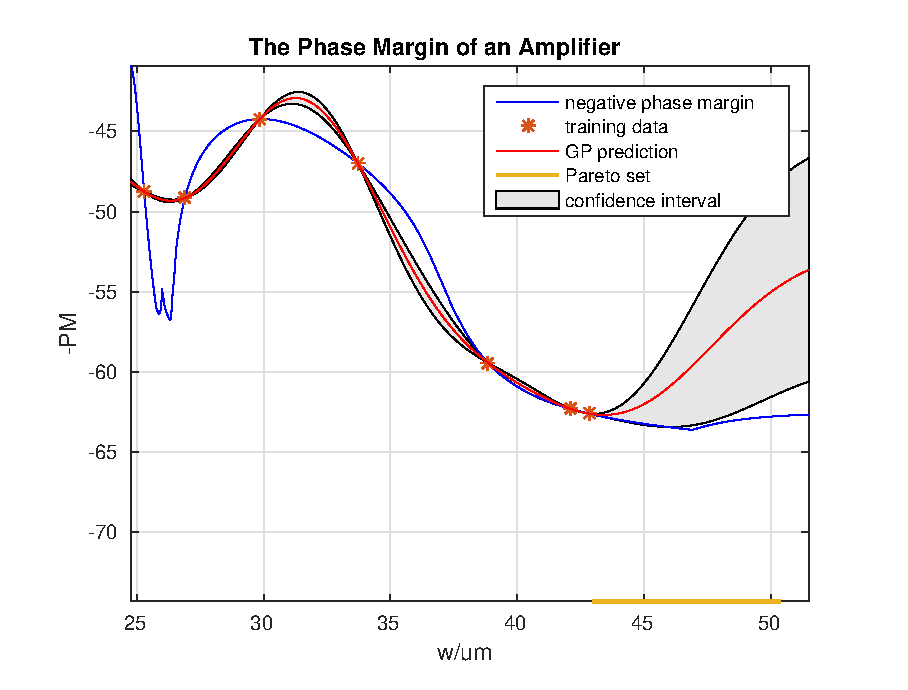
\includegraphics[width=0.36\textwidth]{./img/pm_gp_ps.eps}
    ~
    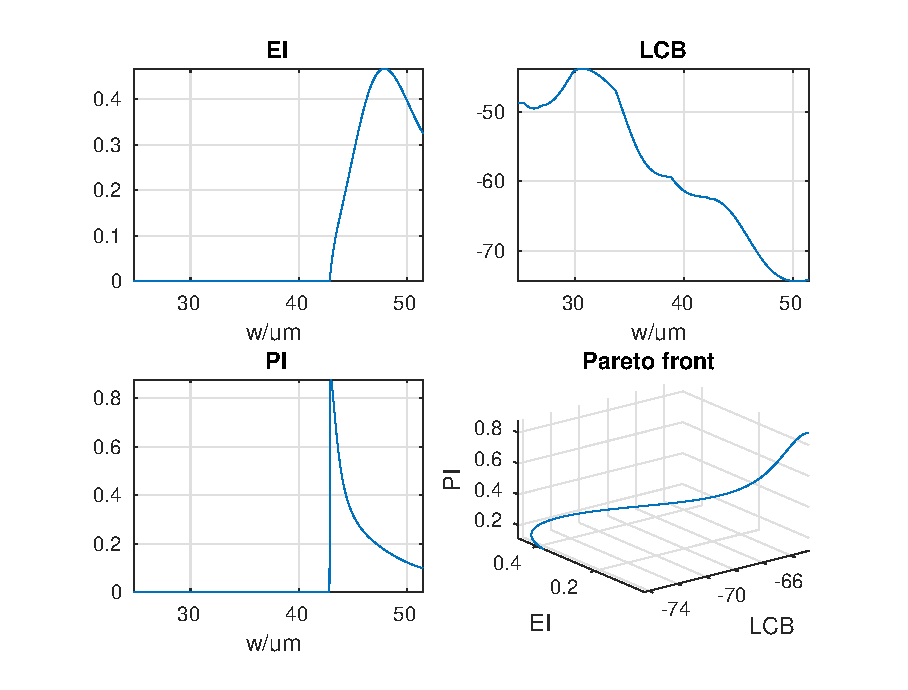
\includegraphics[width=0.36\textwidth]{./img/pf.eps}

    New points are selected from the Pareto set (the yellow points) of the acquisition functions
    }

}


  \headerbox{Results of Benchmark Functions}{name=Benchmark,column=1,span=2, below=MACE, above=bottom}{
      \center{
  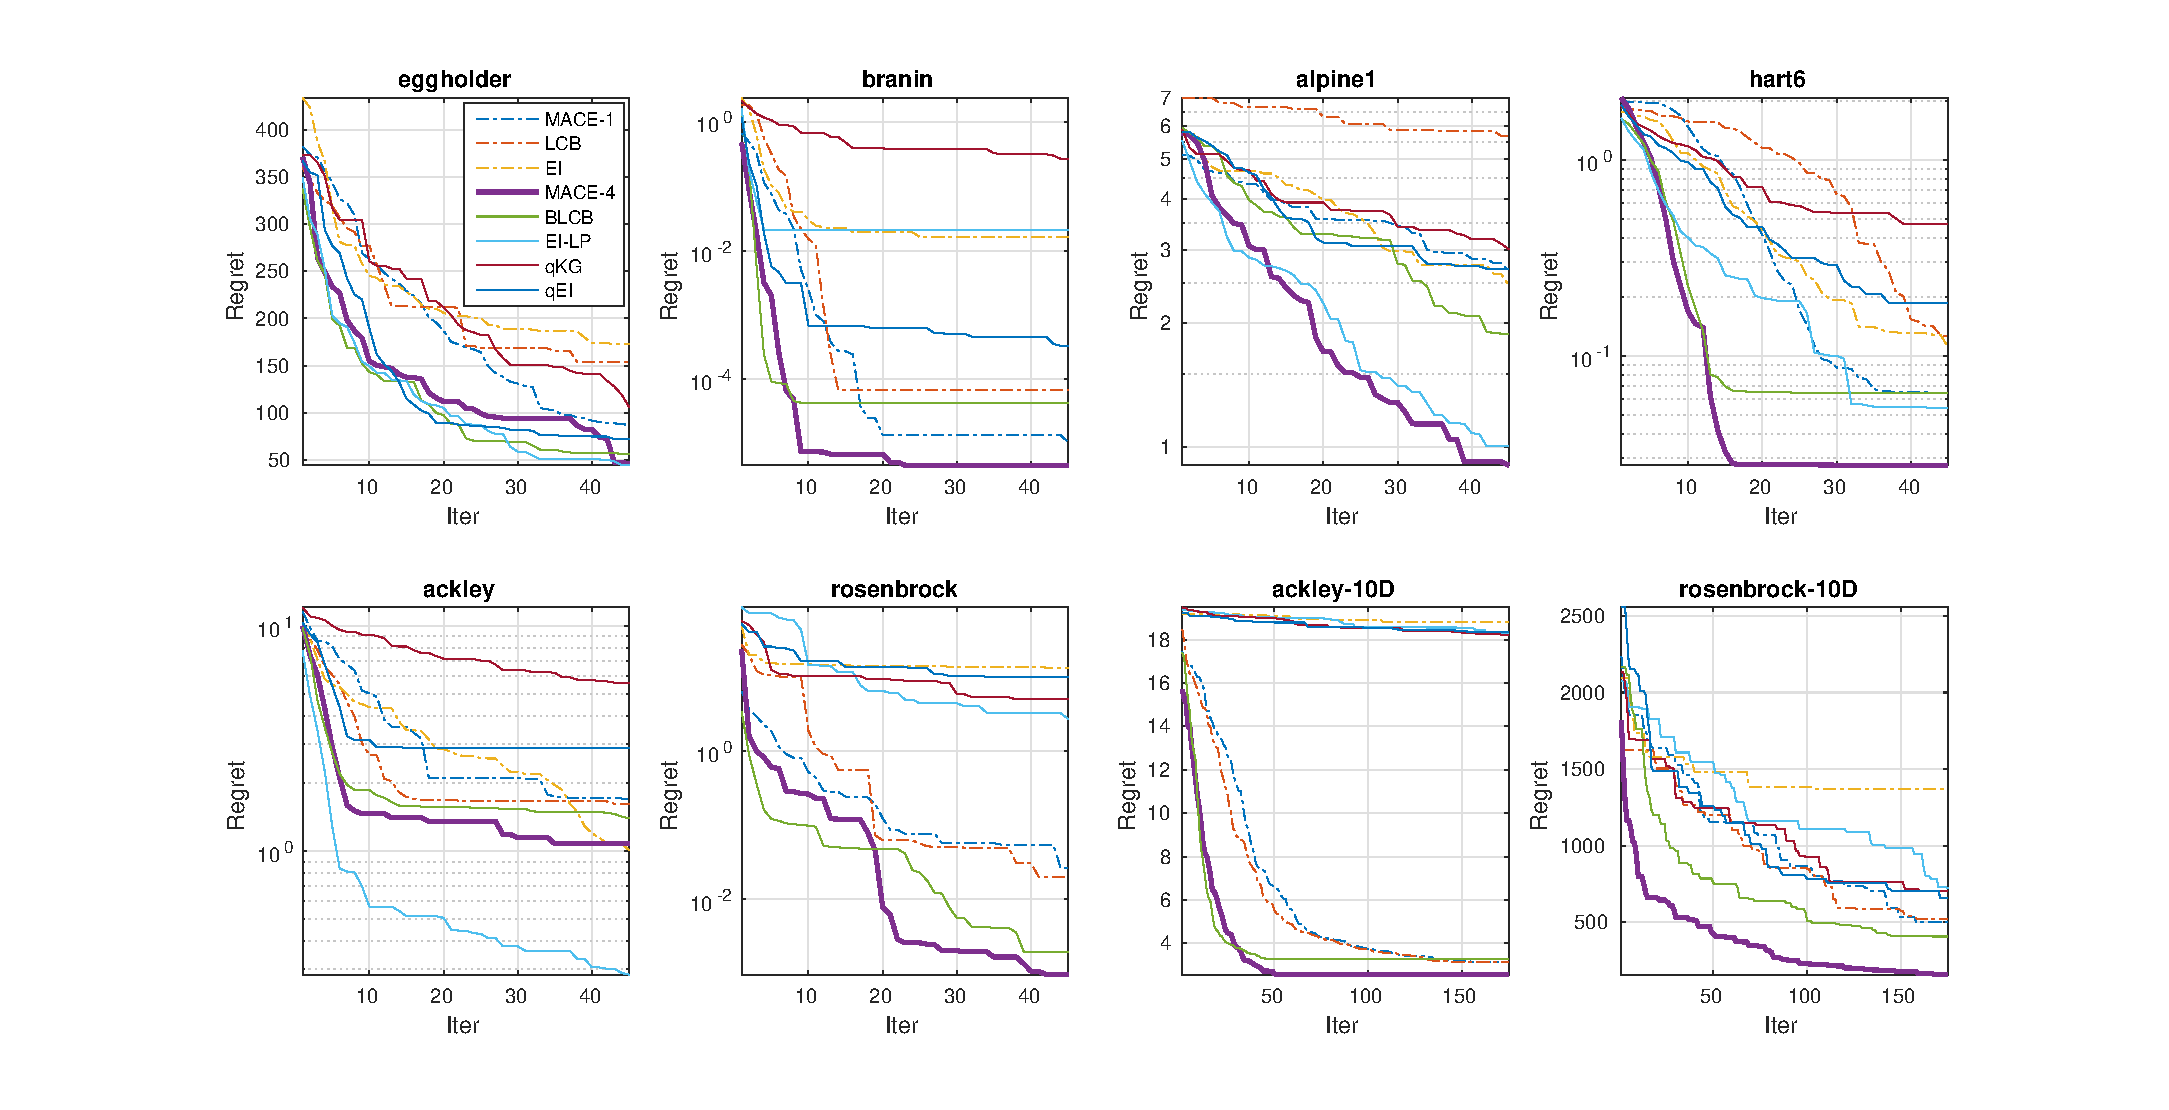
\includegraphics[width=0.82\linewidth]{./img/convplot.eps}
  }
          
  Dotted lines: optimization result with batch size $B$=1. Solid lines: optimization results with batch size $B$=4

    % \subfigure[]{\label{fig:PF_example_1}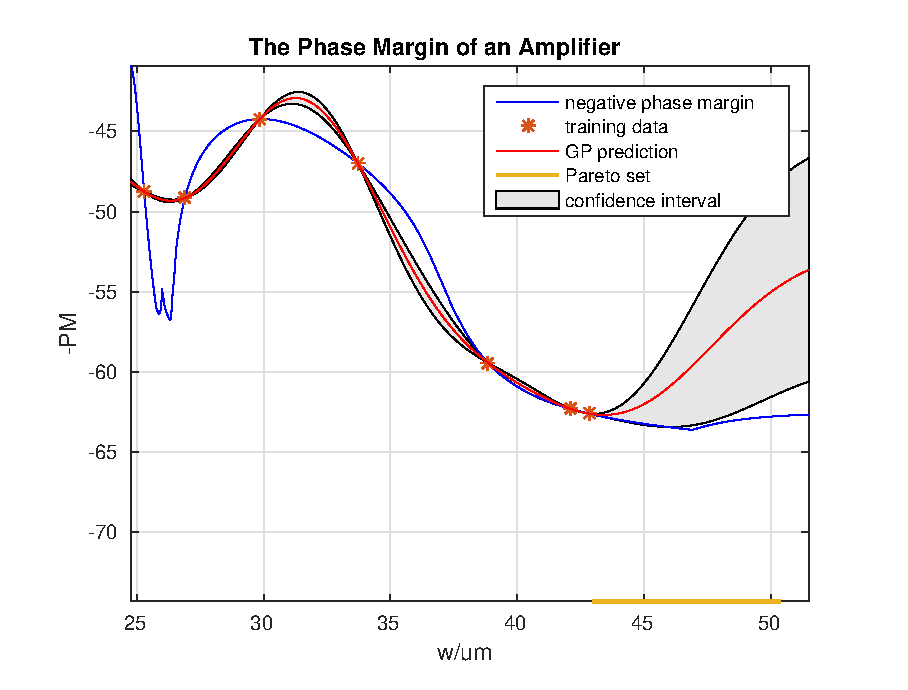
\includegraphics[width=0.49\textwidth]{./img/pm_gp_ps.eps}}
    % ~
    % \subfigure[]{\label{fig:PF_example_2}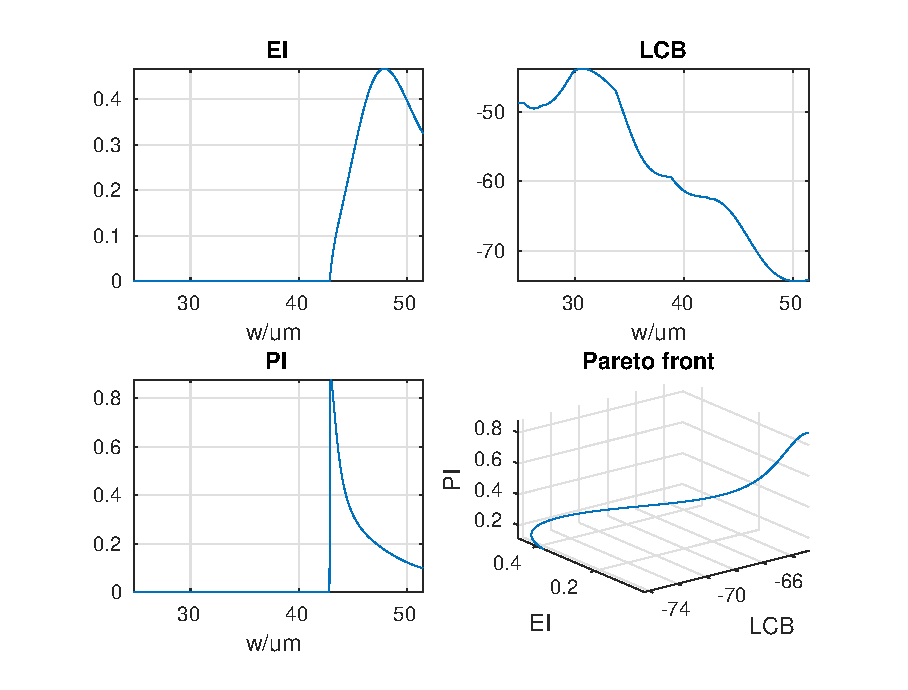
\includegraphics[width=0.49\textwidth]{./img/pf.eps}}
    % \label{fig:PF_example}
% \end{figure}

    % \caption{Optimization results of the benchmark functions}
    % \label{fig:CovPlotBenchmark}
}

  \headerbox{Schematic of the OpAmp Circuit}{name=schopamp,column=3,span=1, row=0}{
      \centerline{\includegraphics[width=0.60\linewidth]{./img/sopam.pdf}}
  }
  \headerbox{Results of the OpAmp circuit}{name=opamp,column=3,span=1, below=schopamp}{
      \centerline{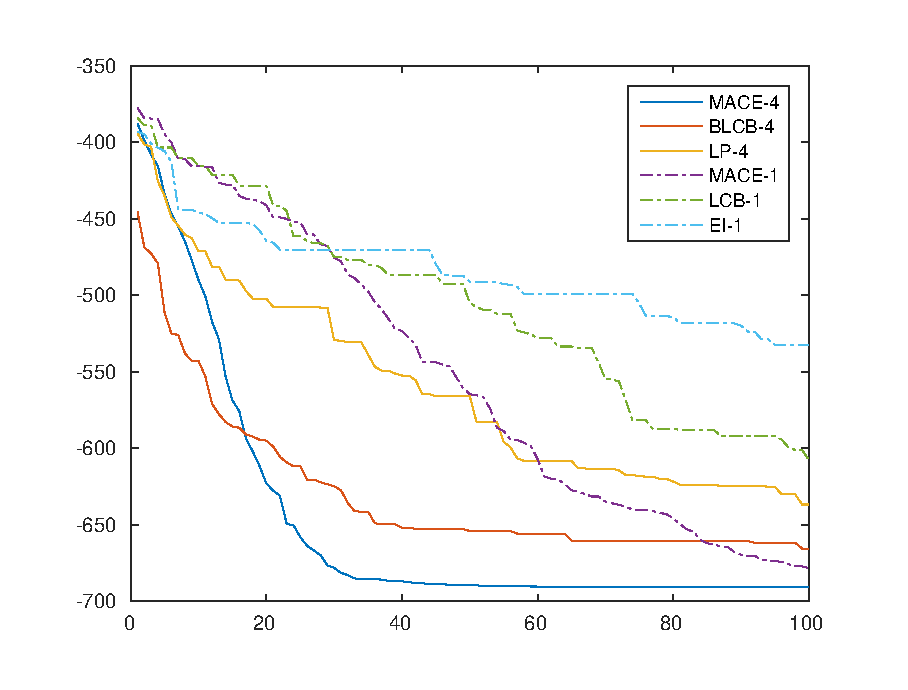
\includegraphics[width=0.60\linewidth]{./img/mean_DAC2014.eps}}
  }
  \headerbox{Schematic of the Power Amplifier}{name=schpa,column=3,span=1, below=opamp}{
      \centerline{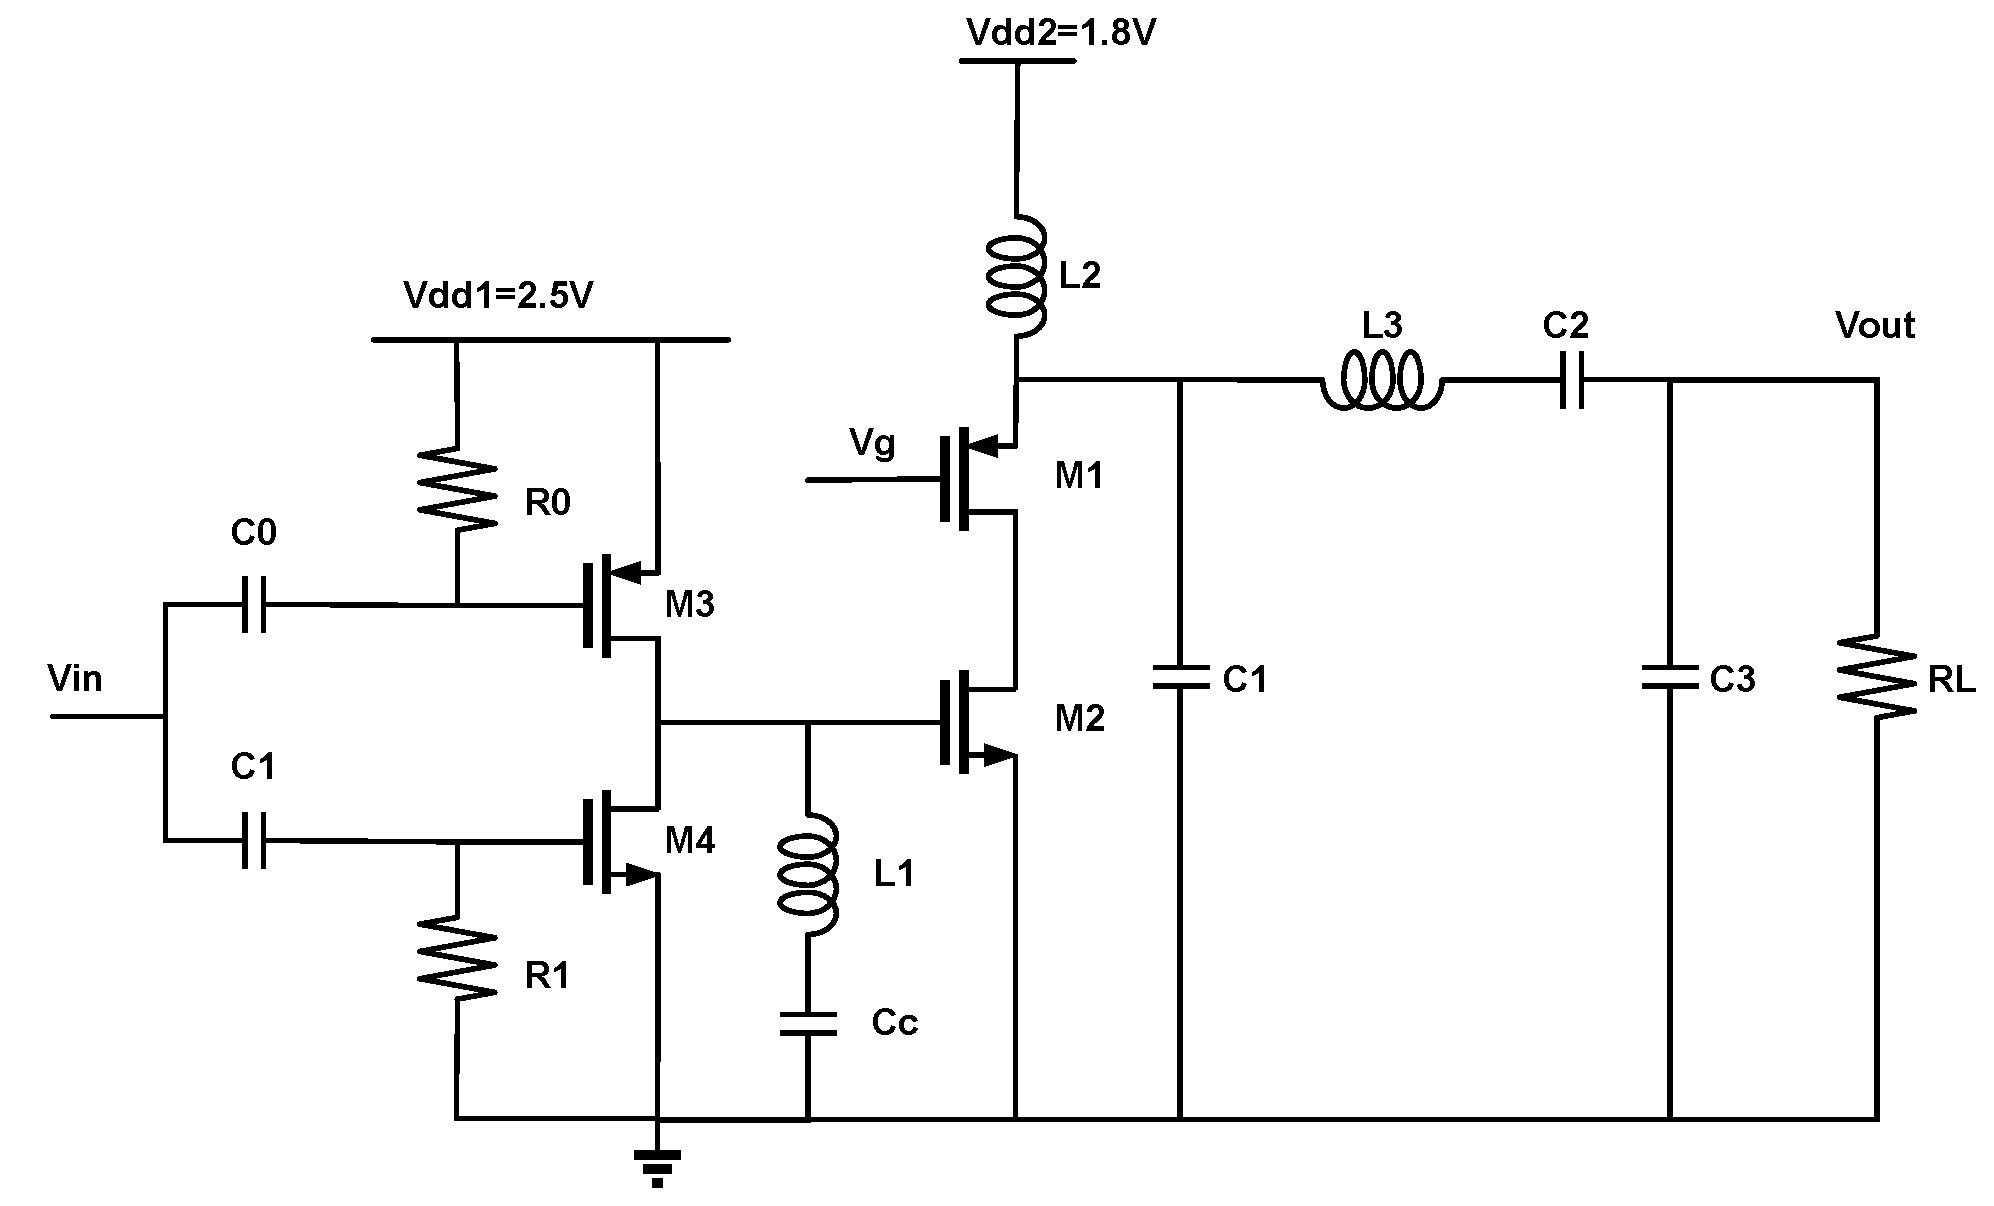
\includegraphics[width=0.60\linewidth]{./img/classE.eps}}
  }
  \headerbox{Results of the power amplifier}{name=PA,column=3,span=1, below=schpa}{
      \centerline{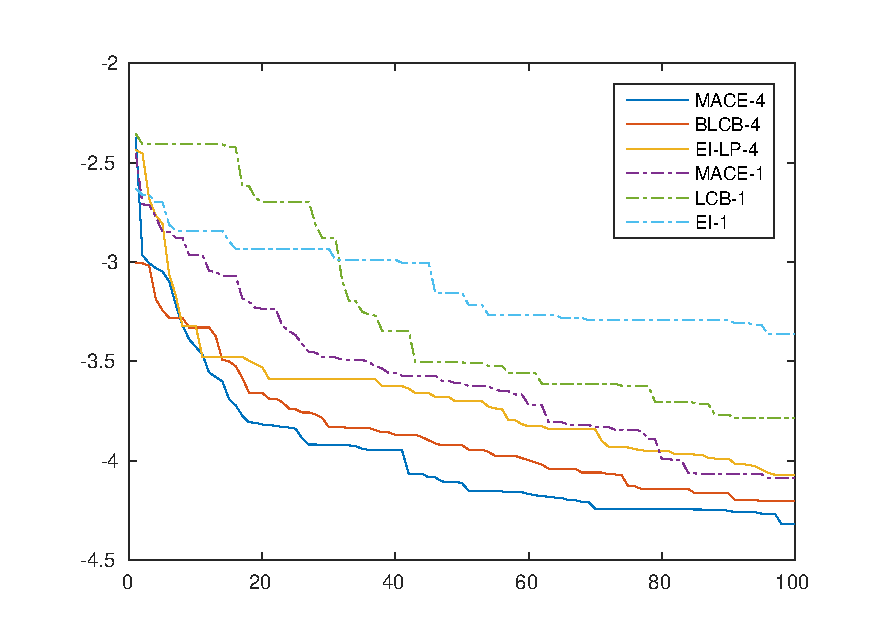
\includegraphics[width=0.60\linewidth]{./img/ClassE_mean.eps}}
}

\end{poster}
%
\end{document}
